\subsubsection{Power Calculation}
We assume that up to rated power, the rotation of each wind turbine can be controlled such that a constant power coefficient of 0.42 is achieved. The wind turbine power generation is defined as:
\begin{equation}
P = 
\begin{cases} 
      C_P\frac{1}{2}\rho V_{\text{eff}}^3A & V_{\text{eff}}\leq V_{\text{rated}} \\
      P_{\text{rated}} & V_{\text{eff}} > V_{\text{rated}}
   \end{cases}
\end{equation}
\noindent Where $C_P$ is the power coefficient, $\rho$ is the air density which we assumed was 1.1716 kg m$^{-3}$, $A$ is the swept area of the turbine rotor, and $V_{\text{eff}}$ is an effective wind speed across rotor, which is defined as:
\begin{equation}
V_{\text{eff}} = V(1-L)
\end{equation}
\noindent Where $V$ is the free stream wind speed at the turbine hub height, and L is the total velocity deficit.
%It is defined as an area-weighted average of the wind speeds across the rotor:
%Katie: Is it a weighted area? or is it a weighted average? If the area is weighted, then you need a hypen (area-weighted average). 

%\begin{equation}
%V_{\text{eff}} = \frac{\int_A V dA }{A}
%\end{equation}

%\noindent Again, in this equation, only the hub height velocities are considered. There is no vertical integration of the wind speed across the rotor hub. The wind shear is considered only in calculating the free stream wind speed.
%Katie:Why is this? Why not do vertical integration? Out of your scope? Ignore this if you talk about this earlier in the paper, as I've jumped to methodology. 


\subsubsection{Wind Speed Distributions}

%We used two different empirical wind distributions; first we used wind data from the city of Alturas, California, second we used data from the Princess Amalia Wind Farm, off the coast of the Netherlands. 
%Katie: It almost seems as if this wind farm is both in the Netherlands and in California. You could either say. "from the city of Alturas, California and from the Princess Amalia Wind Farm, a wind farm off the coast of the Netherlands." OR "from both the Princess Amalia Wind Farm, a wind farm off the coast of the Netherlands, and the city of Alturas, California."
%The data we have is separated into 36 bins every 10 degrees, and 72 bins every 5 degrees, respectively. Both wind roses are shown in Section \ref{sec:optimization}, Fig. \ref{wind_roses}.
%, and the Princess Amalia wind rose is shown in Figure \ref{amalia}. 

%\begin{figure}[htbp]
 % \centering
  %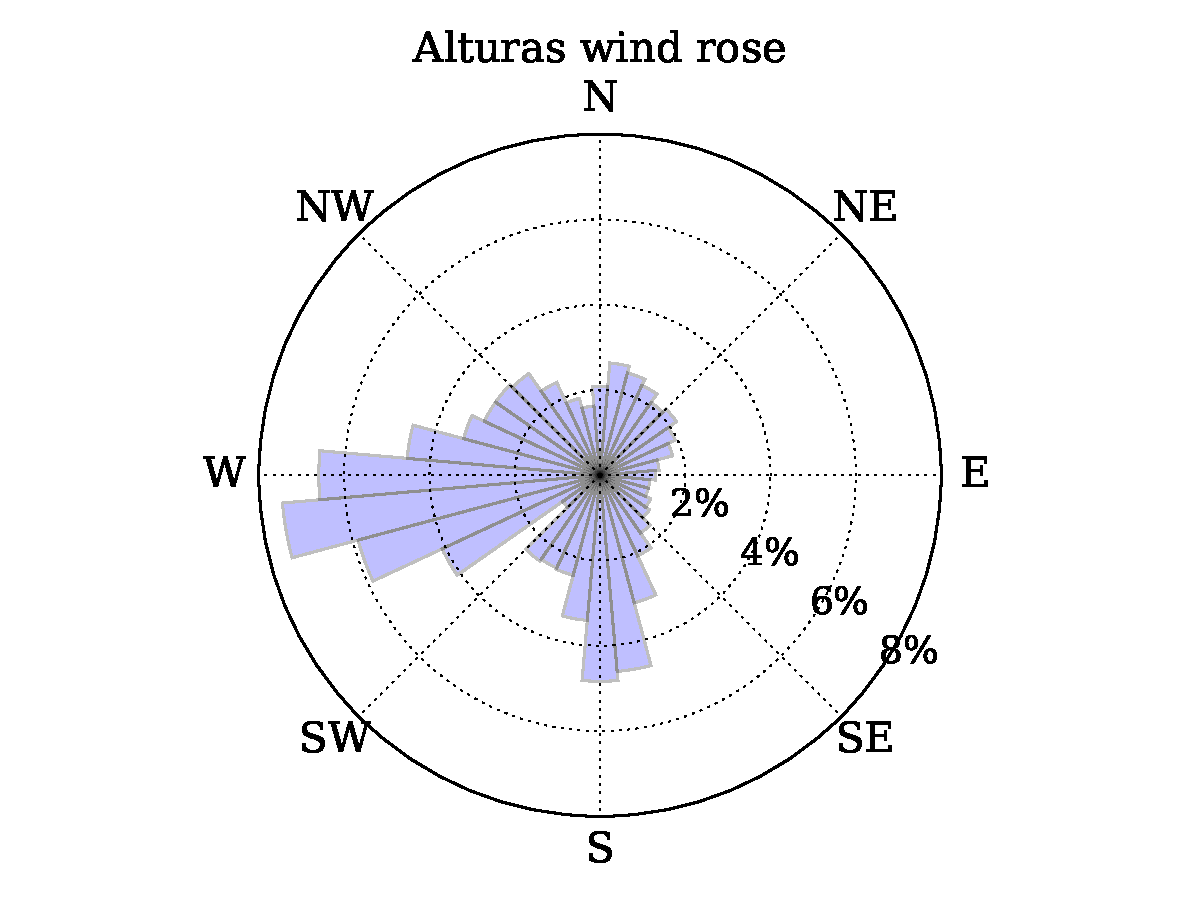
\includegraphics[width=0.49\textwidth]{Figures/alturas_rose.pdf}
  %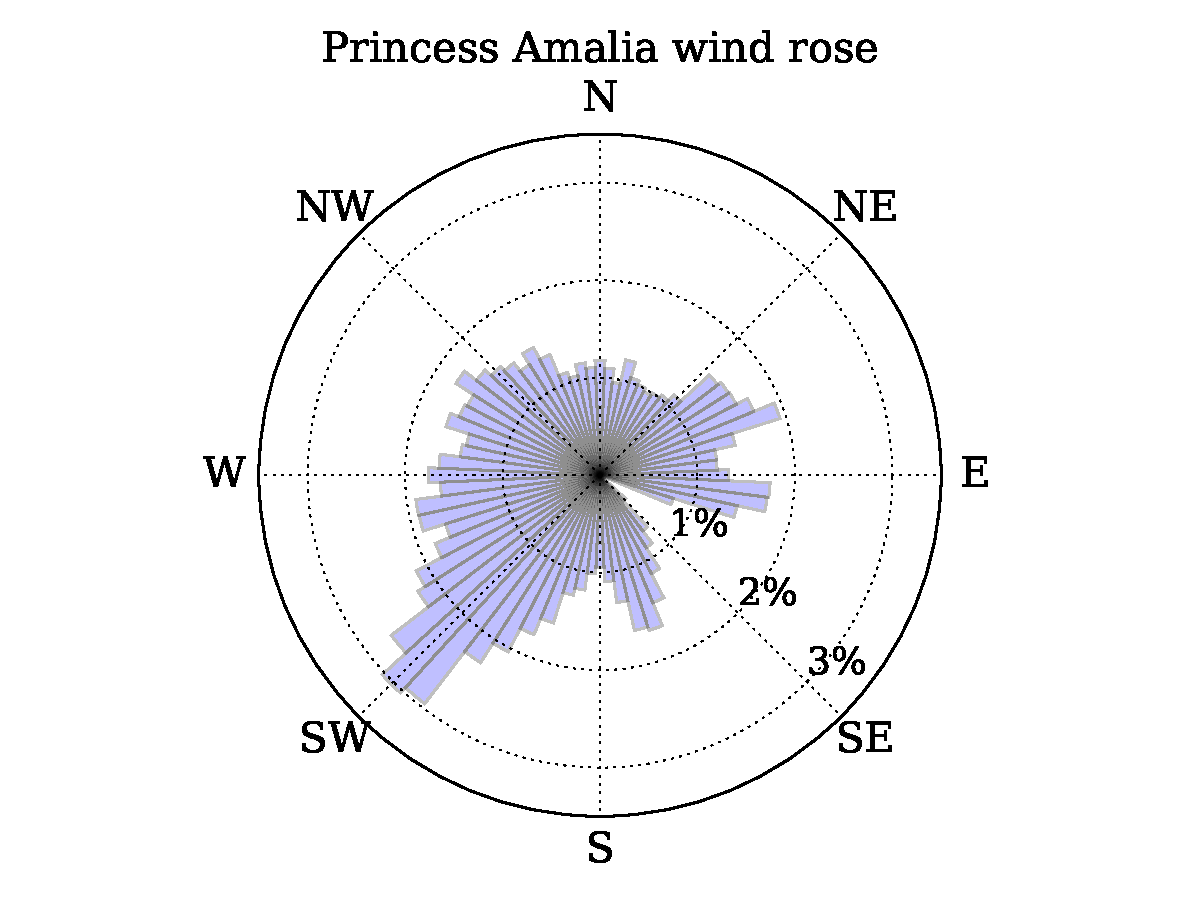
\includegraphics[width=0.49\textwidth]{Figures/amalia_rose.pdf}
  %\caption{\label{wind_roses} On the left, the wind direction distribution in Alturas, California, separated into 36 bins, every 10 degrees. On the right, the wind direction distribution of the Princess Amalia Wind Farm, separated into 72 bins, every 5 degrees.}
%\end{figure}

%\begin{figure}[htbp]
  %\centering
  %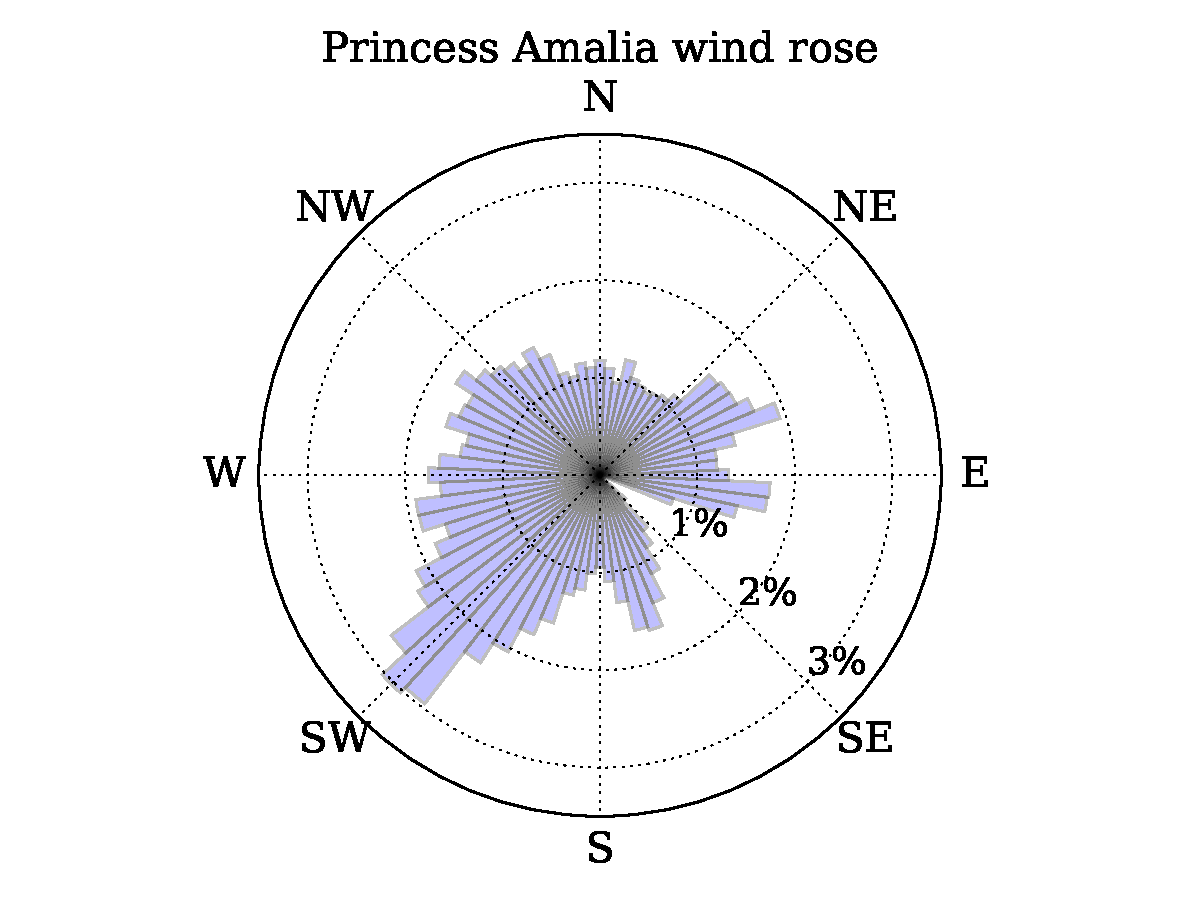
\includegraphics[width=0.75\textwidth]{Figures/amalia_rose.pdf}
  %\caption{\label{amalia} The wind direction distribution of the Princess Amalia Wind Farm, separated into 72 bins, every 5 degrees.}
%\end{figure}

%Just as wind direction varies, the wind speed at any direction also changes. 
We represented the speeds at any wind direction as a Weibull distribution, which is commonly used to represent wind speed distributions \citep{justus1978methods,rehman1994weibull,dorvlo2002estimating}: 
\begin{equation}
W(x) = \Big(\frac{k}{V_{\text{mean}}}\Big)\Big(\frac{x}{V_{\text{mean}}}\Big)^{k-1}\text{exp}\Big[\Big(-\frac{x}{V_{\text{mean}}}\Big)^k\Big]
\end{equation}
The shape factor, $k$, was set as 1.76. 
The mean speed for a given distribution, $V_{\text{mean}}$, can be different depending on the wind direction, meaning that each wind direction has an associated Weibull curve defining the wind speed distribution from that direction. 
%The average speeds, $V_{\text{mean}}$, from every direction for each wind rose are shown in Section \ref{sec:optimization}, Fig. \ref{wind_speeds}.
%The average speed, $V_{\text{mean}}$, for each Weibull distribution is the average wind speed defined for every direction of each wind rose, meaning that each wind direction has an associated Weibull distribution defining the wind speeds from that direction. The average wind speeds from every direction for each wind rose are shown in Section \ref{sec:optimization}, Fig. \ref{wind_speeds}.
Figure \ref{weibull} shows the wind speed Weibull distributions for two different $V_{\text{mean}}$ values. 
%Because of a lack of reliable wind speed data for the Alturas wind rose, it is assumed to have an average wind speed of eight meters per second, which is uniform across all wind directions. For the Princess Amalia Wind Farm, $V_{\text{mean}}$ is defined as the directionally averaged wind speed for each wind direction (thus each direction has a different $V_{\text{mean}}$).
%for each wind direction is defined as the average wind speed from each wind direction. 
%These directionally averaged wind speeds are shown in Fig. \ref{amalia_speeds}. 

%\begin{figure}[htbp]
 % \centering
  %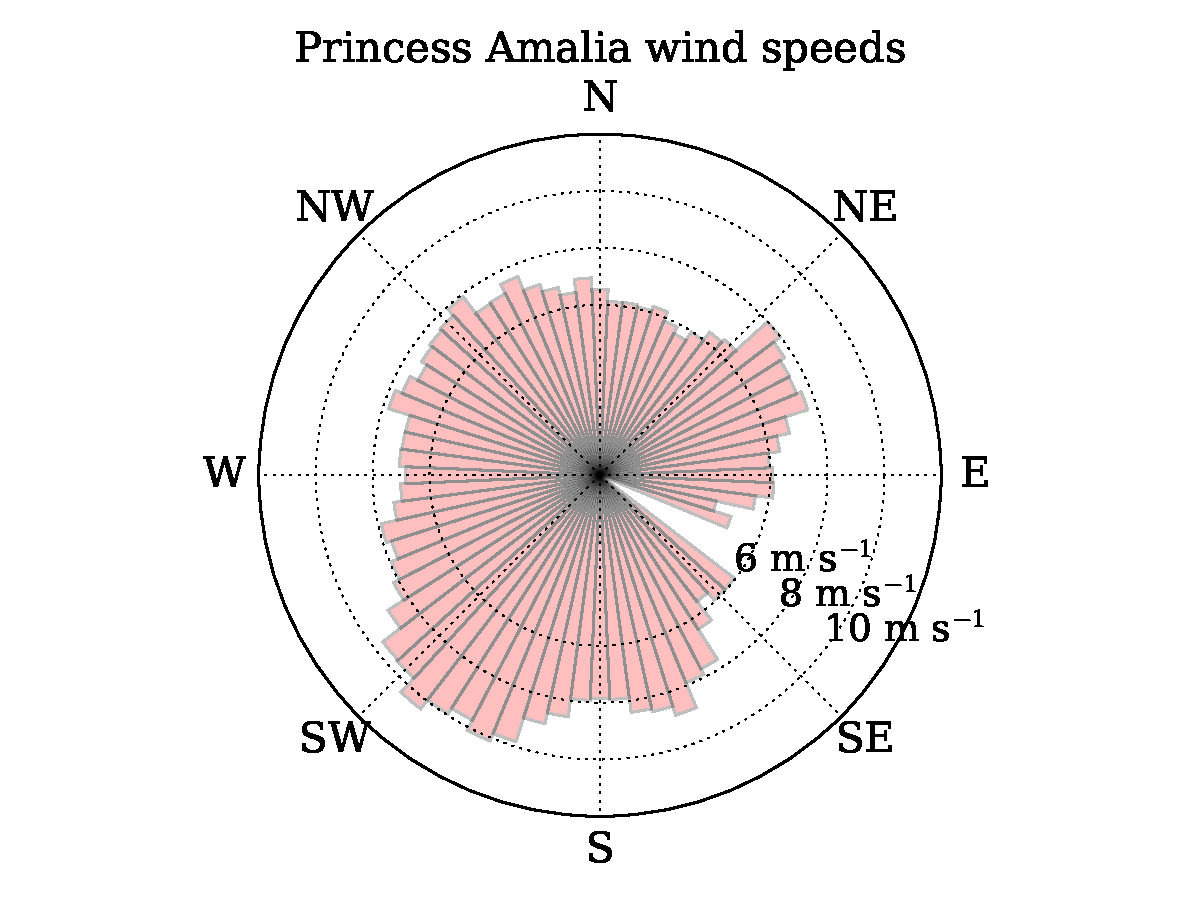
\includegraphics[width=0.49\textwidth]{Figures/amalia_speeds.pdf}
  %\caption{\label{amalia_speeds} The directionally averaged wind speeds of the Princess Amalia Wind Farm, separated into 72 bins, every 5 degrees.}
%\end{figure}
%Katie: Maybe this is obvious to people reading your paper, but why is the shape factor set at 1.76?

\begin{figure}[htbp]
  \centering
  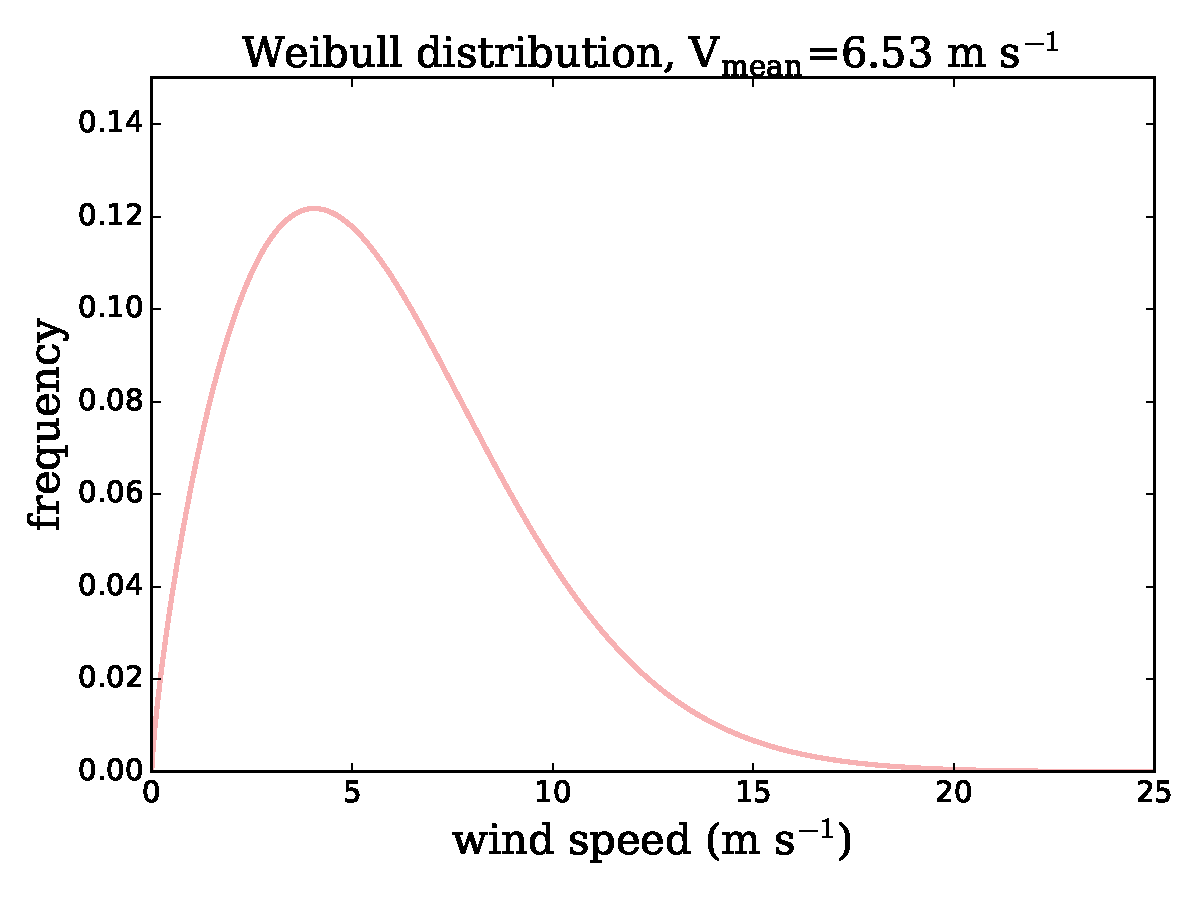
\includegraphics[width=0.4\textwidth]{Figures/weibull_6_53.pdf}\label{653}
  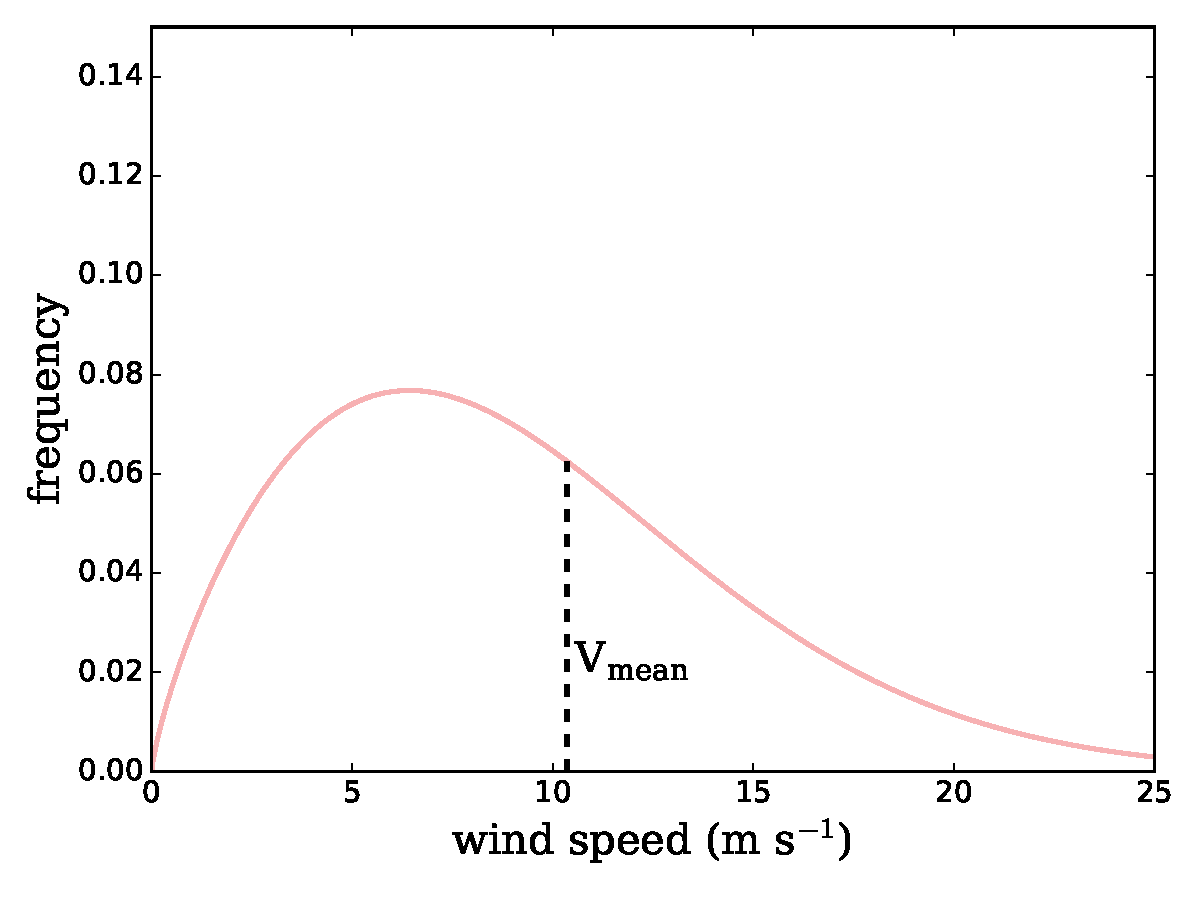
\includegraphics[width=0.4\textwidth]{Figures/weibull_10_35.pdf}\label{1035}
 % \subfloat[]{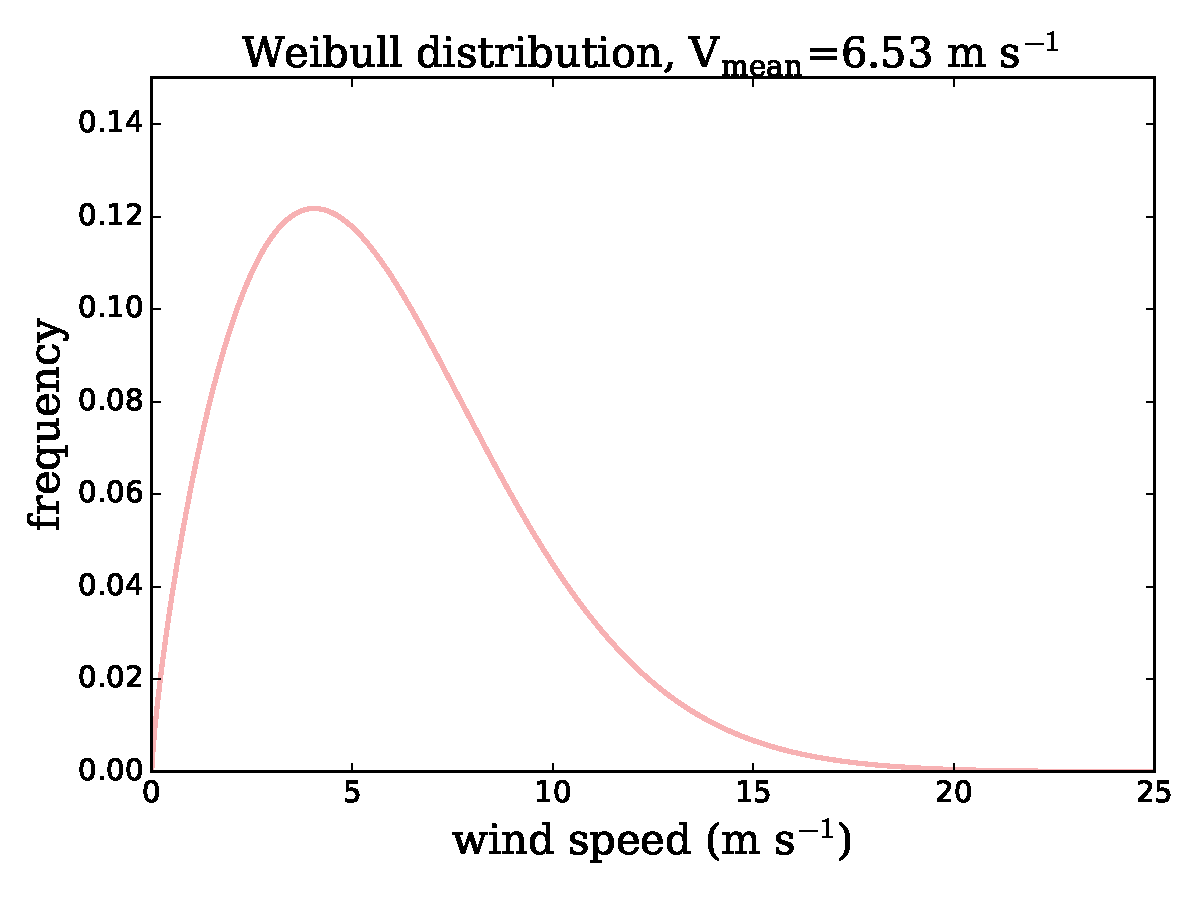
\includegraphics[width=0.5\textwidth]{Figures/weibull_6_53.pdf}\label{653}}
  %\subfloat[]{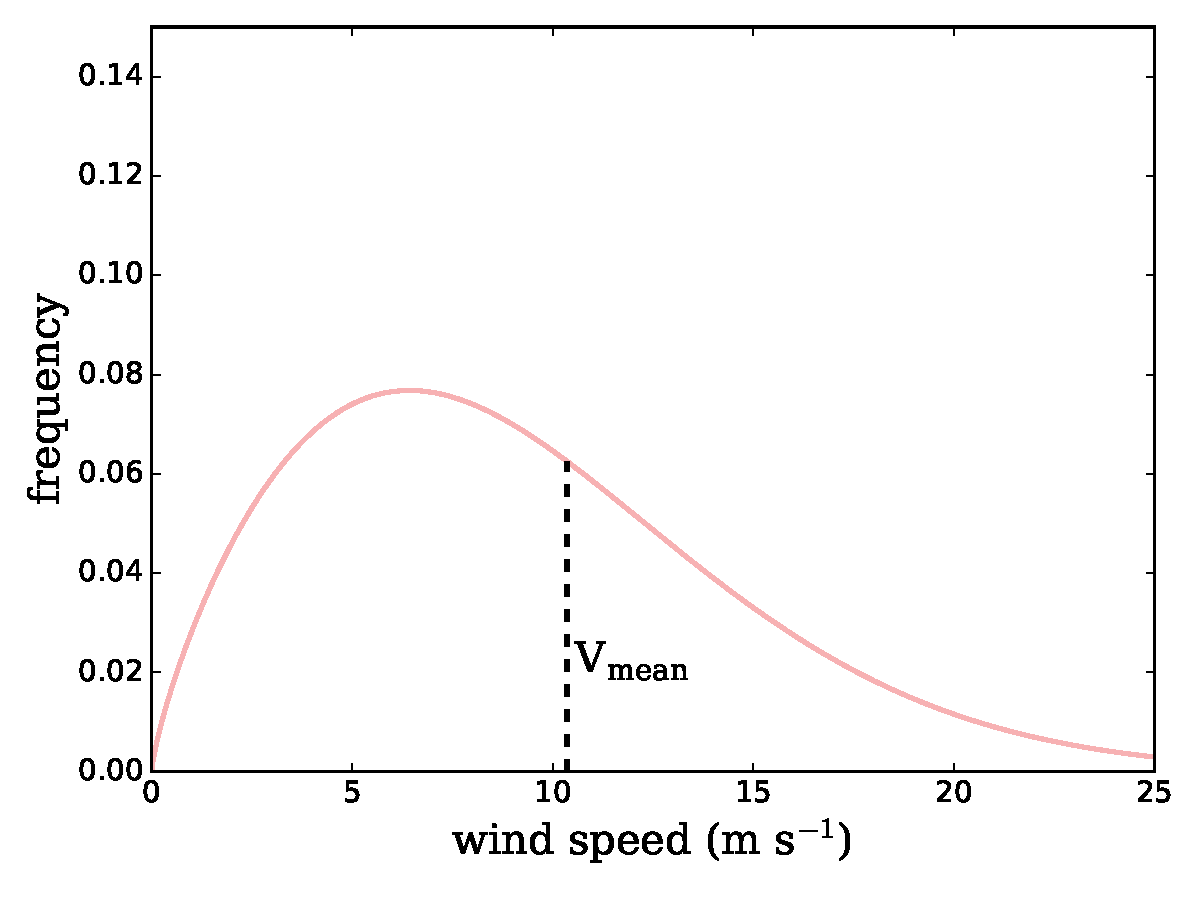
\includegraphics[width=0.5\textwidth]{Figures/weibull_10_35.pdf}\label{1035}}
  \caption{\label{weibull} The Weibull wind speed distributions for two different average wind speeds. In (a) there is an average wind speed of 6.53 meters per second, and (b) shows an average wind speed of 10.35 meters per second. The shape factor k in each Weibull distribution is chosen as 1.76.}
\end{figure}
%Katie: Why didn't you use a Weibull distribution for the California wind? Also you have misspelled distribution in Figure 5.



\subsubsection{Sampling}
The direction data we have is binned into 36 directions for one wind rose, and 72 directions for the other. This is very fine sampling,
%Katie: Why spell out seventy two but leave 36? Is that part of your style guide? If not, choose one and remain consistent throughout the paper. 
from a convergence study, we found that it is more refined than necessary to accurately compute the annual energy production (AEP) of a wind farm. 
%Katie: Then why do fine sampling? Or are you saying that you didn't use all these bins? This part confused me a bit. 
For every wind direction at which the power is computed, the wake model must be called; therefore, reducing the number of directions at which the wind farm power is computed will reduce the time required to optimize. 
%Katie: Consider instead: Reducing the number of directions at which the wind farm power is computed will reduce the time required to optimize because  the wake model must be called for every wind direction at which the power is computed. 
However, too few directions and the AEP calculation will be inaccurate. We fit a spline to the direction data and were thus able to sample at any direction. We then performed a two-dimensional convergence study to find how many directions and speeds were required to approach the ``true'' AEP, which we defined to be the AEP calculated when using 50 wind directions and 30 wind speed samples. 
%Katie: The wording of the last sentence is odd and took me a while to figure it out. Also, you move between present tense and past tense in this entire methodologies section. Choose one. Also in the part "close to the true AEP" how close is close? Consider instead: We then performed a two dimensional convergence study to find how many directions and speeds were required to be almost equivalent to the ``true'' AEP. We found that 50 wind direction samples and 30 wind speed samples were necessary. However,
We found that at 23 wind direction samples and 5 wind speed samples from the Weibull distributions, the AEP converged within 2\% of the true AEP. This is within the error of our wake model; therefore, this number of samples was used in our study. 
%Katie: "this number of samples was used in our study, instead of the higher numbers that came slightly closer to true AEP. 